%!TEX root = slides.tex

\section{Languages}

\begin{frame}{Popular programming languages}
  \begin{description}
    \item[JavaScript] ``high-level, dynamic, untyped, and interpreted''
    \item[SQL] ``special-purpose programming language''
    \item[Java] ``general-purpose, concurrent, class-based, object-oriented''
    \item[C\#] ``multi-paradigm programming language''
    \item[PHP] `` server-side scripting''
    \item[Python] ``high-level, general-purpose, interpreted, dynamic''
    \item[C++] ``general-purpose, imperative, object-oriented and generic''
    \item[C] ``general-purpose, imperative''
    \item[Node.js?] ``open-source, cross-platform JavaScript runtime environment''
  \end{description}
  \citeurl{stackoverflow.com/research/developer-survey-2015}
\end{frame}


\begin{frame}{Kinds of programming languages}
  \begin{description}
    \item[Interpreted] Software interprets the language at runtime. 
    \item[Compiled] Software translates the language into machine code, which is then run.\\[1cm] 
    \item[Systems] Designed with operating system, device drivers development in mnid.
    \item[Applications] Designed with user applications development in mind.\\[1cm]
    \item[High-level] Abstration from the nitty-gritty computer details.
    \item[Imperative] Statements change the program state.
  \end{description}
\end{frame}


\begin{frame}{Styles}
  \begin{center}
    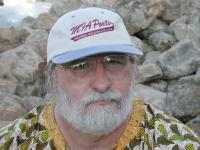
\includegraphics[width=1.4in]{img/richard-gabriel.jpg}
  \end{center}
  \begin{quote}
    I'm always delighted by the light touch and stillness of early programming languages.
    Not much text; a lot gets done.
    Old programs read like quiet conversations between a well-spoken research worker and a well studied mechanical colleague, not as a debate with a compiler.
    Who'd have guessed sophistication bought such noise? \\
    \hspace*\fill{\small--- Dick Gabriel}
  \end{quote}

  \citeurl{web.stanford.edu/class/ee380/Abstracts/100428-pike-stanford.pdf}
\end{frame}

\begin{frame}{People: Dennis Ritchie}
  \begin{figure}
  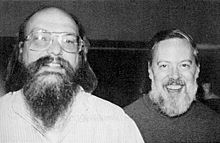
\includegraphics{img/ritchie-thompson.jpg}
  \caption*{Dennis Ritchie 1941-2011 (right)}
  \end{figure}
\end{frame}



\section{Go}
\begin{frame}[fragile]{Hello, World!}
  \begin{minted}{go}
package main
import "fmt"
func main() {
  fmt.Println("hello world")
}
  \end{minted}
  \citeurl{gobyexample.com/hello-world}
\end{frame}
